\documentclass[10pt, xcolor=x11names, compress]{beamer}
%\documentclass[10pt, xcolor=x11names, compress, handout]{beamer}
\usetheme{progressbar}
%\usecolortheme[named=Purple4]{structure}
\progressbaroptions{headline=sections,titlepage=normal,frametitle=normal}

\setbeamertemplate{navigation symbols}{}

\usepackage{iwona} 

\usepackage{alltt}
\usepackage{amsmath,amsfonts, amssymb, amscd}
\usepackage{hyperref}
\usepackage{setspace}
\usepackage{wasysym}
\usepackage{ulem}

\usepackage{calc}
\usepackage[overlay,absolute]{textpos}
\TPGrid[5mm,5mm]{20}{20}



\renewcommand{\Re}{\operatorname{Re}}
\renewcommand{\Im}{\operatorname{Im}}
\newcommand{\debye}{\operatorname{debye}}

\newcommand{\chik}{$\chi(k)$}
\newcommand{\chir}{$|\tilde{\chi}(R)|$}


\newcommand{\file}[1]{{\color{Firebrick4}\texttt{`#1'}}}
\newcommand{\multiple}{{\color{Orange3}\textsl{multiple}}}


\newcommand{\atoms}  {{\color{DarkOrchid4}\textsc{atoms}}}
\newcommand{\feff}   {{\color{DarkOrchid4}\textsc{feff}}}
\newcommand{\ifeffit}{{\color{DarkOrchid4}\textsc{ifeffit}}}
\newcommand{\athena} {{\color{DarkOrchid4}\textsc{athena}}}
\newcommand{\artemis}{{\color{DarkOrchid4}\textsc{artemis}}}

\renewenvironment<>{center}
{\begin{actionenv}#1\begin{originalcenter}}
{\end{originalcenter}\end{actionenv}}

\definecolor{guessp}   {rgb}{0.64,0.00,0.64}
\newcommand{\guessp}   {{\color{guessp}guess}}
\definecolor{defp}     {rgb}{0.00,0.55,0.00}
\newcommand{\defp}     {{\color{defp}def}}
\definecolor{setp}     {rgb}{0,0,0}
\newcommand{\setp}     {{\color{setp}set}}
\definecolor{lguessp}  {rgb}{0.24,0.11,0.56}
\newcommand{\lguessp}  {{\color{lguessp}lguess}}
\definecolor{skipp}    {rgb}{0.70,0.70,0.70}
\newcommand{\skipp}    {{\color{skipp}skip}}
\definecolor{restrainp}{rgb}{0.80,0.61,0.11}
\newcommand{\restrainp}{{\color{restrainp}restrain}}
\definecolor{afterp}   {rgb}{0.29,0.44,0.55}
\newcommand{\afterp}   {{\color{afterp}after}}
\definecolor{penaltyp} {rgb}{0.55,0.35,0.17}
\newcommand{\penaltyp} {{\color{penaltyp}penalty}}
\definecolor{mergep}   {rgb}{0.93,0.00,0.00}
\newcommand{\mergep}   {{\color{mergep}merge}}


\mode<presentation>

\title{Prospects for Synchrotron Environmental Science}
\author{Bruce Ravel}
\institute[NIST]{Synchrotron Methods Group, Ceramics
  Division\\Materials Science and Engineering Laboratory\\National
  Institute of Standards and Technology}
\date[UDel, 22-09-08]{University of Delaware\\September 22, 2008}

\begin{document}
\maketitle

\begin{frame}
  \frametitle{Copyright}
  \tiny

  This document is copyright \copyright 2007-2010 Bruce Ravel.

  \begin{center}
    
\includegraphics[width=1.0cm]{images/somerights20}
  \end{center}

  This work is licensed under the Creative Commons
  Attribution-ShareAlike License.  To view a copy of this license,
  visit \href{http://creativecommons.org/licenses/by-sa/3.0/}
  {\color{Purple4}\texttt{http://creativecommons.org/licenses/by-sa/3.0/}}
  or send a letter to Creative Commons, 559 Nathan Abbott Way,
  Stanford, California 94305, USA.

  \begin{description}
  \item[You are free:] %
    \begin{itemize}
    \item \textbf{to Share} --- to copy, distribute, and transmit the work
    \item \textbf{to Remix} --- to adapt the work
    \end{itemize}
  \item[Under the following conditions:] %
    \begin{itemize}
    \item Attribution. You must attribute the work in the manner
      specified by the author or licensor (but not in any way that
      suggests that they endorse you or your use of the work).
    \item Share Alike. If you alter, transform, or build upon this
      work, you may distribute the resulting work only under the same,
      similar or a compatible license.
    \item Any of these conditions can be waived if you get permission
      from the author.
    \end{itemize}
  \end{description}
  \begin{itemize}
  \item For any reuse or distribution, you must make clear to others
    the license terms of this work. The best way to do this is with a
    link to the URL for this document.
  \item Any of the above conditions can be waived if you get
    permission from the copyright holder.
  \item Nothing in this license impairs or restricts the author's
    moral rights.
  \end{itemize}

  Your fair dealing and other rights are in no way affected by the
  above.  This is a human-readable summary of the Legal Code (the full
  license).


\end{frame}

%%% Local Variables:
%%% mode: latex
%%% TeX-master: "pimst2"
%%% End:


\section[Introduction]{Introduction}

%\subsection{Beamline}
\begin{frame}
  \frametitle{This Talk}
  
  This talk is presents my view of new opportunities for synchrotron
  environmental science with a substantial bias towards inner-shell
  spectroscopy (XAS, XRF, etc.).

  \bigskip

  \begin{block}{Outline}
    \begin{itemize}
    \item An brief review of X-ray Absorption Spectroscopy
    \item An overview of the novel capabilities of NSLS-II
    \item Some examples of science that can be done at third
      generation synchrotron sources
    \end{itemize}
  \end{block}

  \bigskip

  My intent is to get everyone in the room thinking creatively about
  what synchrotron experiments they might be doing in the next 10-15
  years.
\end{frame}

\subsection[Synchrotron Radiation]{Synchrotron Radiation}

\begin{frame}
  \frametitle{Synchrotron radiation, briefly}

  \begin{center}
    \small
    Electrons traveling near the speed of light are contained in a
    storage ring.  Specialized magnets accelerate the electrons,
    generating x-rays.

    \smallskip

    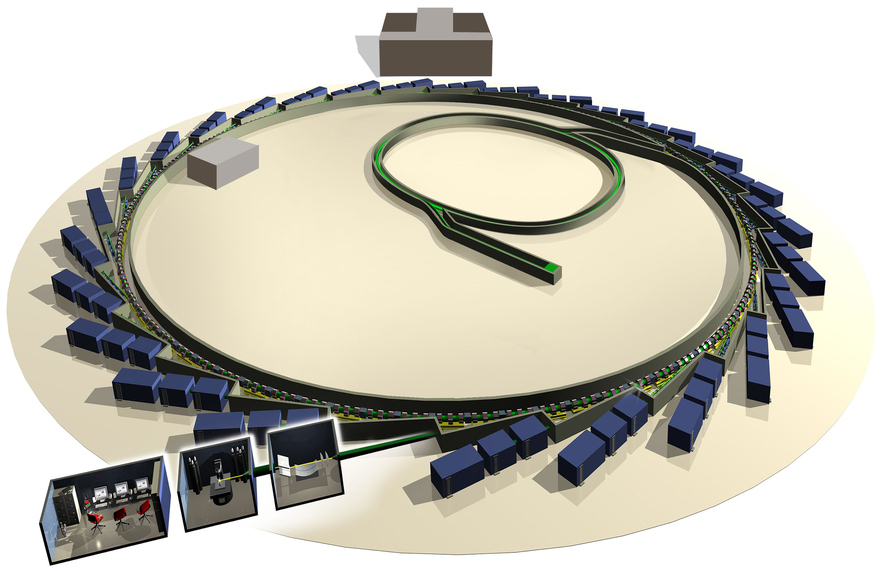
\includegraphics[width=0.8\linewidth]{pses/DLS008h_sm.jpg}

    \smallskip

    The x-rays are conditioned by optics and directed into a
    hutch were experiments can be performed.
  \end{center}
  \begin{textblock*}{0.5\linewidth}(0pt,19.5\TPVertModule) 
    \tiny
    image from lightsources.org
  \end{textblock*}
\end{frame}

\begin{frame}
  \frametitle{Why use a synchrotron?}

  \begin{center}
    \alert{Answer:} Intensity and brightness!
  \end{center}
  \begin{columns}
    \begin{column}{0.5\linewidth}
      Shown here is the on-axis brilliance of various sources.

      Even at the K$\alpha$ energy, an anode is down by 5 to 9 orders
      of magnitude compared to a synchrotron source.
    \end{column}
    \begin{column}{0.5\linewidth}
      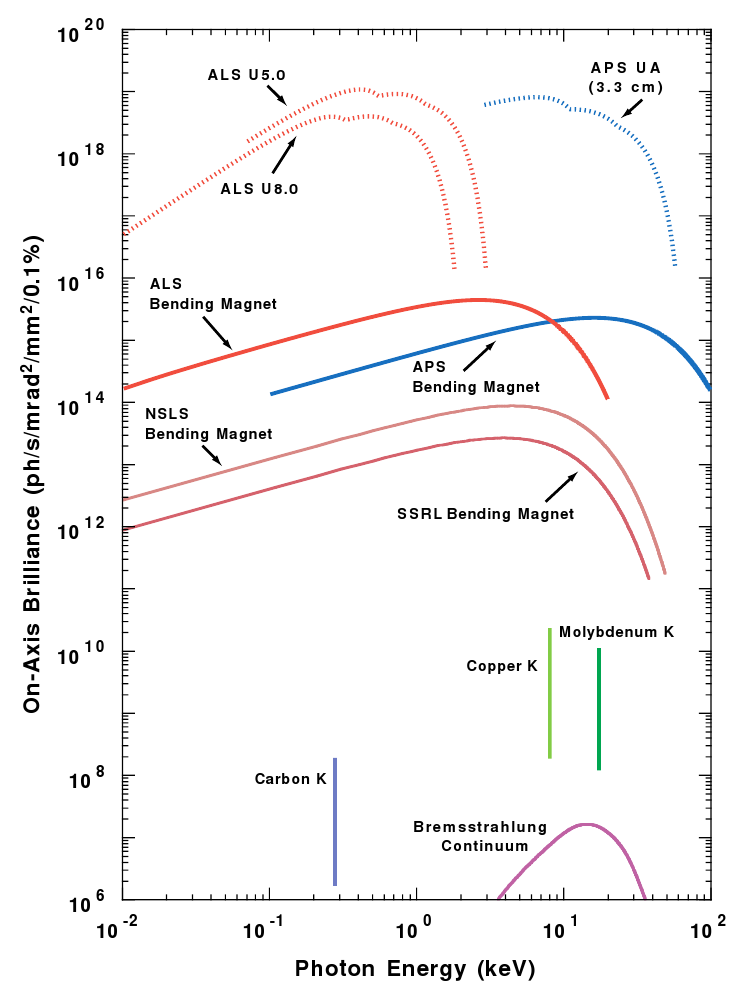
\includegraphics[width=\linewidth]{pses/nsb0898_616.png}
    \end{column}
  \end{columns}
  \begin{textblock*}{0.5\linewidth}(0pt,19.5\TPVertModule) 
    \tiny
    image from J.R. Helliwell, \textit{Synchrotron radiation facilities},
    \textit{Nature Structural Biology}  \textbf{5}, 614 - 617 (1998)
  \end{textblock*}
\end{frame}


\subsection[Spectroscopy]{Inner Shell Spectroscopy}

\setbeamercovered{dynamic}
%\setbeamercovered{transparent=50}

\begin{frame}
  \frametitle{The physical process in X-ray Absorption
    Spectroscopy and X-Ray Fluorescence}

  \begin{center}
\only<beamer| beamer:1>{\includegraphics[width=0.7\linewidth]{images/atom.pdf}}%
\only<beamer| beamer:2>{\includegraphics[width=0.7\linewidth]{images/ion.pdf}}%
\only<beamer| beamer:3>{\includegraphics[width=0.7\linewidth]{images/emission.pdf}}
    \only<handout>{
      \includegraphics[width=0.33\linewidth]{images/atom.pdf}
      \includegraphics[width=0.33\linewidth]{images/ion.pdf}
      \includegraphics[width=0.33\linewidth]{images/emission.pdf}
    }
  \end{center}

  %\vskip -25pt

  \begin{enumerate}[<+->]
  \item An incoming photon interacts with a deep-core electron.  Shown
    here, a 1s electron is excited for a K-edge spectrum.
  \item The deep-core electron is promoted to some unoccupied state
    above the Fermi energy, propagates away, and leaves behind a
    core-hole.
  \item A short time later (1 or 2 femtoseconds), a higher-lying
    electron decays into the core-hole and emits a photon.
  \end{enumerate}
\end{frame}

% \begin{frame}
%   This page needs to explain that we change the incident energy and
%   measure the absorption cross section.
% \end{frame}

\begin{frame}
  \frametitle{XAS and Valence State}

  \begin{columns}
    \begin{column}{0.5\linewidth}
      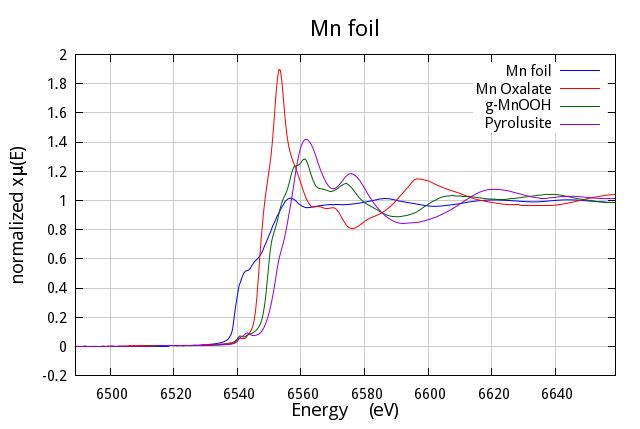
\includegraphics[width=\linewidth]{xas/mn_xanes.png}
    \end{column}
    \begin{column}{0.5\linewidth}
      As the valence increases\\[1ex]

      {\color{Blue3}Mn$^0$}$\rightarrow$ 
      \alert{Mn$^{2+}$} $\rightarrow$
      {\color{Green4}Mn$^{3+}$} $\rightarrow$
      {\color{Purple3}Mn$^{4+}$}\\[1ex]

      the edge position shifts to higher energy.
    \end{column}
  \end{columns}    

  \bigskip

  \begin{block}{XAS is a direct measure of valence state}
    \begin{itemize}
    \item Since each element has its own edge energy, an element's
      valence can be measured even in a heterogeneous sample
    \item Since x-rays are deeply penetrating into matter, minimal
      sample preparation is required
    \item No assumption of symmetry or periodicity is made, so the
      sample can be crystalline, amorphous, thin film, in solution,
      surface sorbed, $\cdots$ , \textit{whatever}
    \end{itemize}
  \end{block}

\end{frame}


\begin{frame}
  \frametitle{XAS and Local Atomic Structure}
  \begin{columns}[T]
    \begin{column}{0.34\linewidth}
      \visible<1->{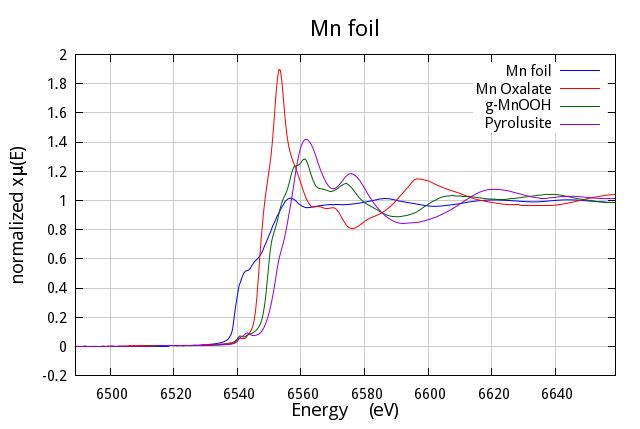
\includegraphics[width=\linewidth]{xas/mn_xanes}}

      \visible<2->{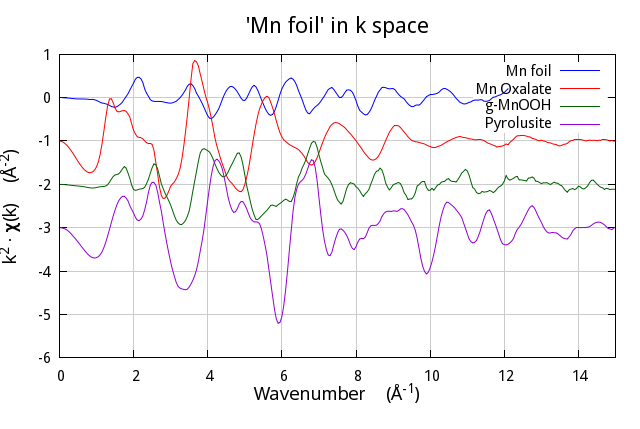
\includegraphics[width=\linewidth]{xas/mn_chik}}

      \visible<3>{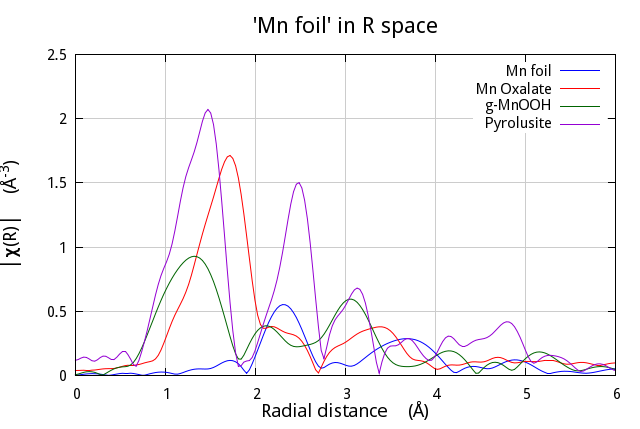
\includegraphics[width=\linewidth]{xas/mn_chir}}
    \end{column}
    \begin{column}{0.66\linewidth}
      \begin{itemize}[<+->]
      \item The different Mn species also show big differences in the
        fine structure beyond the edge as the valence increases
        ({\color{Blue3}Mn$^0$}, \alert{Mn$^{2+}$},
        {\color{Green4}Mn$^{3+}$}, {\color{Purple3}Mn$^{4+}$}).  The
        white line and subsequent osciellations are quite
        different.\\[3ex]
      \item The oscillatory portion of the spectrum can be isolated
        and ...\\[3ex]
      \item ... Fourier transformed.  This FT function can be
        interpreted to yield a partial pair distribution functions of
        atoms about the absorber.  The Mn-O distances are different
        for the \alert{Mn$^{2+}$}, {\color{Green4}Mn$^{3+}$}, and
        {\color{Purple3}Mn$^{4+}$} and clearly different from the
        Mn-Mn distance in {\color{Blue3}Mn metal}.
      \end{itemize}
    \end{column}
  \end{columns}
\end{frame}


\begin{frame}
  \frametitle{XAS is a direct measure of local structure}

  \begin{itemize}
  \item Since each element has its own edge energy, an element's
    local structure can be measured even in a heterogeneous sample
  \item Since x-rays are deeply penetrating into matter, minimal
    sample preparation is required
  \item No assumption of symmetry or periodicity is made, so the
    sample can be crystalline, amorphous, thin film, in solution,
    surface sorbed, $\cdots$ , \textit{whatever}
  \item Samples can be measured \textit{in situ}, which can mean
    \begin{itemize}
    \item cryostat or furnace
    \item high pressure cell
    \item electrochemistry cell or fuel cell
    \item peristaltic or stop-flow pump with liquid samples
    \item high field magnet
    \item etc...
    \end{itemize}
  \end{itemize}

  \begin{exampleblock}{}
    \begin{center}
      As a result, XAS is used in a very broad array of scientific
      disciplines
    \end{center}
  \end{exampleblock}
\end{frame}

\begin{frame}
  \frametitle{Fluorescence from A Sediment Sample}
  \begin{center}
    Here are the XRF spectra with incident beams \alert{above} and
    {\color{Blue4}below} the U L$_{III}$ edge for sediment heavily
    contaminated with uranium.

    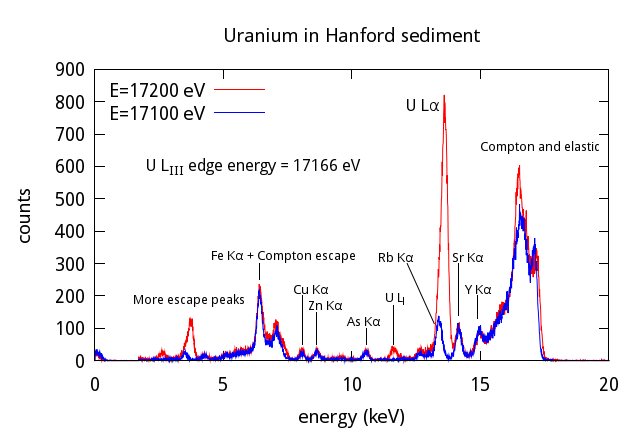
\includegraphics[width=0.7\linewidth]{xrf/xrf.png}
  \end{center}
\end{frame}

\begin{frame}
  \frametitle{X-ray Microscopy}
  
  \begin{columns}
    \begin{column}{0.5\linewidth}
      Microscopy is possible using special focusing optics, such as
      {\color{Blue3}Kirkpatrick-Baez mirror pairs} or
      {\color{Blue3}Fresnel zone plates}.

      \medskip

      \begin{itemize}
      \item Spot sizes of 20 microns are available at NSLS; 1 micron
        and smaller at other sources
      \item Map elemental distribution on that length scale
      \item Microspectroscopy and microdiffraction
      \end{itemize}
    \end{column}
    \begin{column}{0.5\linewidth}
      \begin{center}
        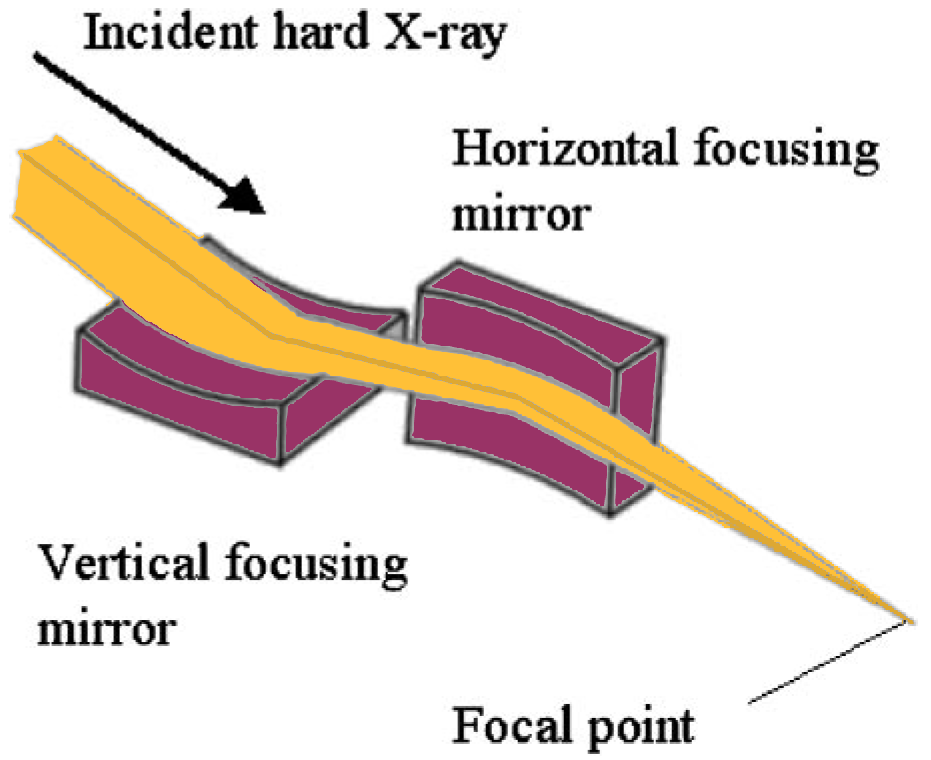
\includegraphics[width=0.9\linewidth]{xrf/kb.png}\\[2ex]
        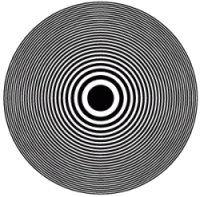
\includegraphics[width=0.6\linewidth]{xrf/zp.png}
      \end{center}
    \end{column}
  \end{columns}
\end{frame}

\section[NSLS-II Overview]{The Capabilities of NSLS-II}

\begin{frame}
  \frametitle{NSLS-II: A big building}
  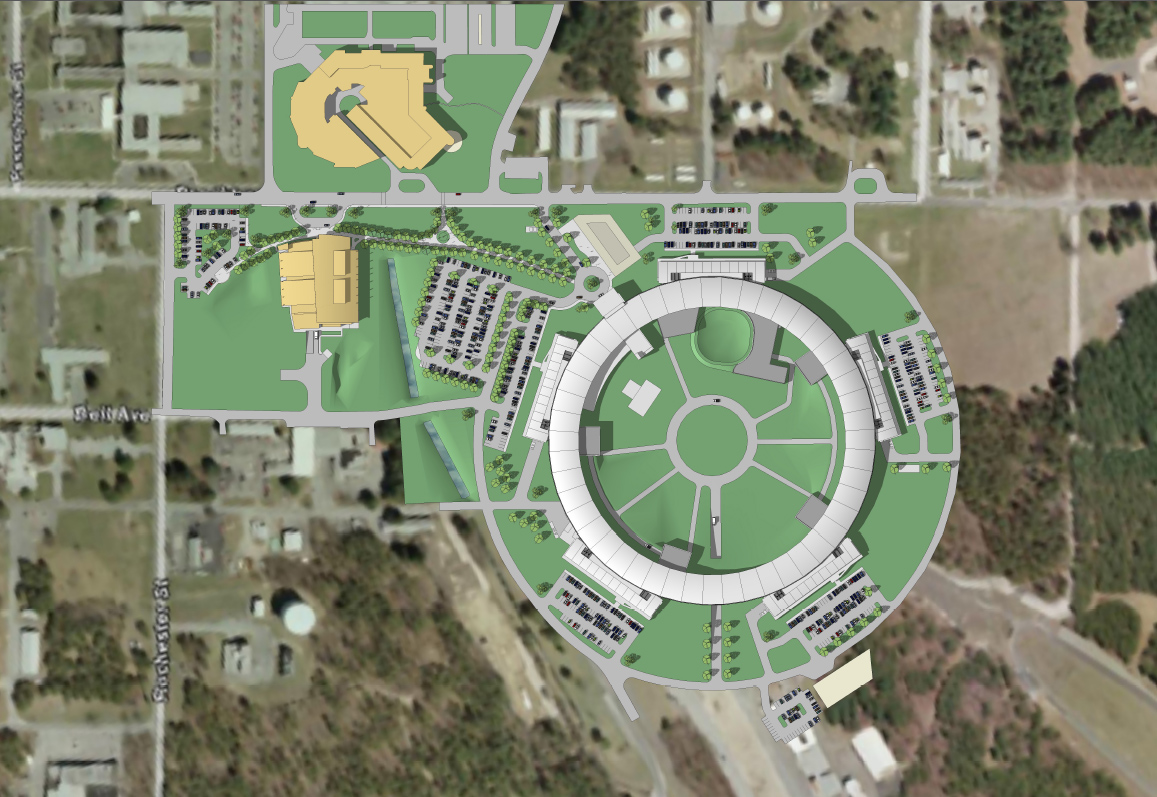
\includegraphics[width=\linewidth]{pses/NSLS2_planView_Jul07-big.jpg}
  \begin{textblock*}{0.5\linewidth}(0pt,19.5\TPVertModule) 
    \tiny
    image from \texttt{http://www.bnl.gov/nsls2/drawings.asp}
  \end{textblock*}
\end{frame}

\begin{frame}
  \frametitle{The big picture}
  \begin{itemize}
  \item 30-sided polygon with a 3-fold symmetric lattice
  \item 28 straight sections + 29 bends (remaining straights used for injection)
  \item $\sim800$ meters in diameter, typical length from source to
    optics is $\sim40$ meters.
  \item Very high brilliance undulators are the standard insertion
    device.  An EPU has been designed.
  \item Several straights must be given up to \alert{damping wigglers}
    to control source divergence.  There is also a design for a
    superconducting wiggler.
  \item Bend magnets have a very low critical energy.  At least four
    will be wide gap devices for extracting IR radiation.
  \item Optional three-pole wigglers can be placed in front of a
    bend.  These will be similar to NSLS bend magnets.
  \end{itemize}
\end{frame}

\subsection[NSLS-II Properties]{NSLS-II Properties}

\begin{frame}
  \frametitle{The first six NSLS-II beamlines}
  The following beamlines will be built using funds from the initial
  construction project:
  \begin{itemize}
    \item Imaging beamlines
    \begin{itemize}
    \item Nanoprobe with a target spot size of $\sim$1\,nm
    \item Microprobe with a target spot size of $\sim$100\,nm
    \end{itemize}
  \item Scattering beamlines
    \begin{itemize}
    \item Inelastic X-ray scattering with 0.1\,meV energy resolution
    \item Soft X-ray coherent scattering
    \item Hard X-ray coherent scattering
    \item Powder diffraction
    \end{itemize}
  \end{itemize}

  \bigskip

  Additional beamlines will follow in later phases of beamline
  development.  
  \begin{itemize}
  \item A second phase of insertion device beamline development is
    planned to follow initial operations by about 1 year.
  \item Resources will be transfered from NSLS to 3PW, soft-bend, and
    IR beamlines.
  \end{itemize}

\end{frame}

\begin{frame}
  \frametitle{What makes NSLS-II special}
  \begin{itemize}
  \item Very small source size (superb for imaging and inelastic scattering)
    \begin{itemize}
    \item Shallow bends (excellent IR and far-IR sources!)
    \item Damping wigglers (high flux up to about 90\,keV)
    \end{itemize}
  \item Long straight sections for insertion devices
  \item 500 mA full current with top-off operations
  \item Extraordinary stability
  \end{itemize}
\end{frame}

\subsection[XAS at NSLS-II]{XAS at NSLS-II}

\begin{frame}
  \frametitle{X-ray absorption spectroscopy on 3-pole and damping wigglers}

  \begin{columns}
    \begin{column}{0.5\linewidth}
      \begin{description}[3-]
      \item [3-pole wigglers] Up to 28 devices with source properties
        quite similar to NSLS bend magnets.
      \item [Damping Wigglers] Initial construction requires 3 sectors
        to be filled with DWs.  The fully instrumented ring may
        require as many as 6.
      \end{description}
    \end{column}
    \begin{column}{0.5\linewidth}
      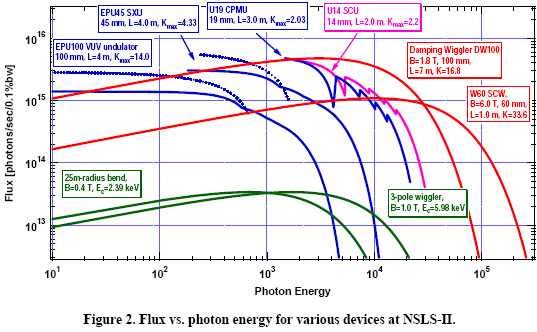
\includegraphics[width=\linewidth]{pses/Src-Prop_Fig-2.png}      
    \end{column}
  \end{columns}
  \begin{block}{Damping Wigglers}
    The DWs represent an area of new possibilities for XAS and other
    inner-shell spectroscopies due to their extraordinarily high flux.
  \end{block}

  \begin{textblock*}{0.5\linewidth}(0pt,19.5\TPVertModule) 
    \tiny
    image from \texttt{http://www.bnl.gov/nsls2/project/source\_properties.asp}
  \end{textblock*}
\end{frame}

\begin{frame}
  \frametitle{The Proposed DWXAS Beamline (I)}
  \includegraphics[width=\linewidth]{pses/XF-BL-XAS-20080314-3.pdf}
\end{frame}
\begin{frame}
  \frametitle{The Proposed DWXAS Beamline (II)}
  \begin{block}{}
    \small
    \begin{tabular}{cccc}
      \textbf{Hutch} & \textbf{spot size} & \textbf{flux (ph/sec)} & 
      \textbf{energy range}\\[2ex]
      %%
      {\color{Blue4}\textbf{EXAFS microprobe}} & $1\,\mu$m & 
      $10^{12}$ & 5.5--25\,keV\\[1ex]
      %% 
      {\color{Blue4}\textbf{Bulk XAS}} & 
      \begin{minipage}{0.2\linewidth}
        $200\,\mu$m (f)\\
        $55\times4$\,mm (u) 
      \end{minipage}
      & 
      $5\times10^{13}$ & 5.5--90\,keV\\[2ex]
      %% 
      {\color{Blue4}\textbf{Tender side station}} & vertical focus & 
      $10^{14}$ & 2.1--6\,keV
    \end{tabular}
  \end{block}
  
  \bigskip

  \begin{itemize}
  \item Best-in-class flux
  \item Slew scanning: XANES in $\sim10$\,sec., EXAFS in $\sim1$\,
    min.
  \item Excellent energy and positional stability
  \item Very large hutches with ample room for special instrumetation
  \item Option for a resolution refining monochromator
  \end{itemize}
  \begin{textblock*}{0.6\linewidth}(0pt,20\TPVertModule) 
    \tiny
    See \texttt{http://xafs.org/NSLSII/XasBeamLine}
  \end{textblock*}
\end{frame}

\section[Novel Science]{Examples of Science Enabled by NSLS-II}

\begin{frame}
  \frametitle{Novel science possibilities at NSLS-II}
  What sorts of experiments can we imagine using capabilities beyond
  those at NSLS?

  \bigskip

  \begin{itemize}
  \item Environmentally relevant metal concentrations
  \item High throughput and sample screening
  \item Energy resolution
  \item Exotic spectroscopies: XES and LERIX
  \end{itemize}

  \bigskip

  Each of these will be discussed with examples of experiments from
  other 3$^{\textrm{rd}}$ generation synchrotrons.
\end{frame}


\subsection[High flux]{High Flux}

\begin{frame}
  \frametitle{Uranium sequestration}

  \small
  \begin{exampleblock}{}
    $\mu$XAS was used to quantify the structure of uranyl
    incorporation into an ancient calcite.  This identifies a
    plausible strategy for uranium sequestration.
  \end{exampleblock}
  \begin{columns}
    \begin{column}{0.6\linewidth}
      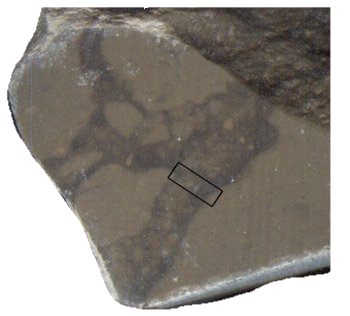
\includegraphics[width=0.4\linewidth]{pses/rock.png}
      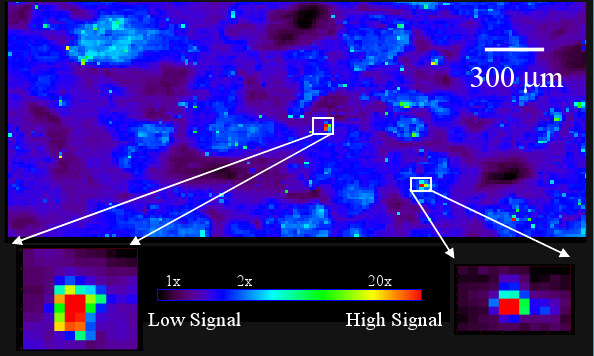
\includegraphics[width=0.6\linewidth]{pses/Umap.png}

      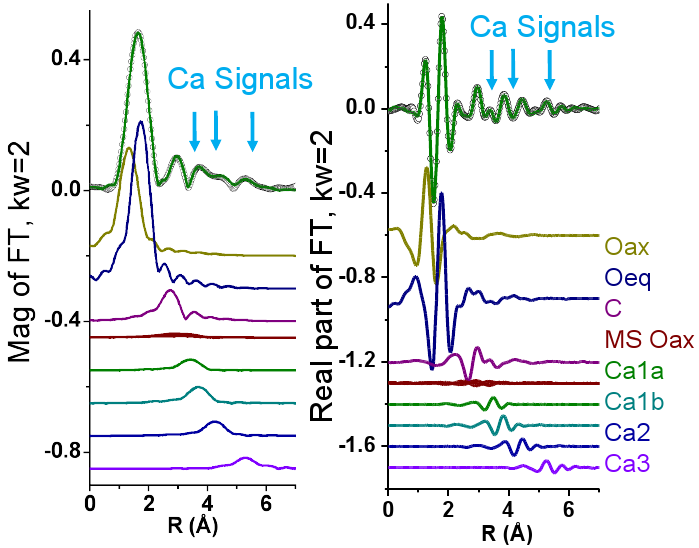
\includegraphics[width=0.6\linewidth]{pses/Uexafs.png}
      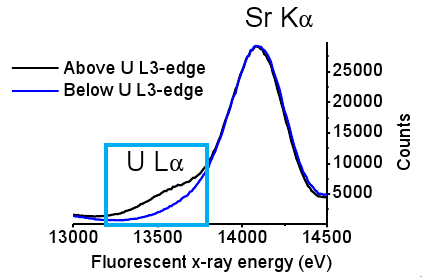
\includegraphics[width=0.4\linewidth]{pses/Ufluo.png}
    \end{column}
    \begin{column}{0.4\linewidth}
      \small
      \begin{itemize}
      \item APS beamline 10ID
      \item $<20$\,ppm U under the spot
      \item 10 $\mu$m spot
      \item Flux: $\sim10^{11}$ ph/sec
      \item 2.5 days of continuous measurement
      \item $\sim2\times10^{16}$ total ph.
      \end{itemize}
    \end{column}
  \end{columns}
  \begin{center}
    \begin{tabular}{lll}
      APS 10ID  & $10^{11}$ ph/sec     & 2.5 days\\
      NSLS X26a & $3\times10^9$ ph/sec & 2.5 months\\
      \alert{NSLS-II DW} & \alert{$10^{12}$ ph/sec} & \alert{6 hours!}
    \end{tabular}
  \end{center}
  \begin{textblock*}{0.6\linewidth}(0pt,20\TPVertModule) 
    \tiny
    S.D.\ Kelly, et al, \textit{Evidence of a stable uranyl site in ancient
    organic-rich calcite}. Environ.\ Sci.\ Technol.\ (2006), \textbf{40}(7),
    2262-2268. 
  \end{textblock*}
\end{frame}

\begin{frame}
  \frametitle{Low concentration and environmental relevance}%%
  \begin{block}{}
    Continued progress in understanding the fate and transport of
    contaminants will require probing of environmentally relevant
    concetrations.
  \end{block}
  \begin{itemize}
  \item Kinetics and speciation at relevant concentration may not be
    well represented by measurement at high concentration
  \item Hg is increasingly important to DOE (e.g.\ extensive Hg
    contamination at Oak Ridge)
  \item Heavy metals (Cd, As, Se, etc) can be taken up in food crops
  \item Probe every stage in a chain of bioaccumulation
  \end{itemize}
  \begin{alertblock}{}
    High flux combined with the ability to probe heterogeneity over
    many length scales is increasingly important.
  \end{alertblock}
\end{frame}

\subsection[High throughput]{High Throughput}

\begin{frame}
  \frametitle{High throughput}

  The materials engineers have pioneered the concept of
  ``combinatorial processing'' wherein samples are presented in a
  plane with parametric gradients in two or three directions.  These
  samples arrays are then measured using automated, high-throughput
  methods.

  \bigskip

  This concept can be adapted to the concerns of environmental science
  for screening samples collected from the field or generated
  parametrically in the lab.

  \bigskip

  \begin{block}{High flux + automation}
    Use high flux and automation of hardware and software to quickly
    screen samples samples:
    \begin{itemize}
    \item Uncover trends in sample sets
    \item Identify samples requiring further study
    \end{itemize}
  \end{block}
\end{frame}

\subsection[Energy resolution]{Energy resolution}

\begin{frame}
  \frametitle{Energy resolution}
  \begin{columns}
    \begin{column}{0.3\linewidth}
      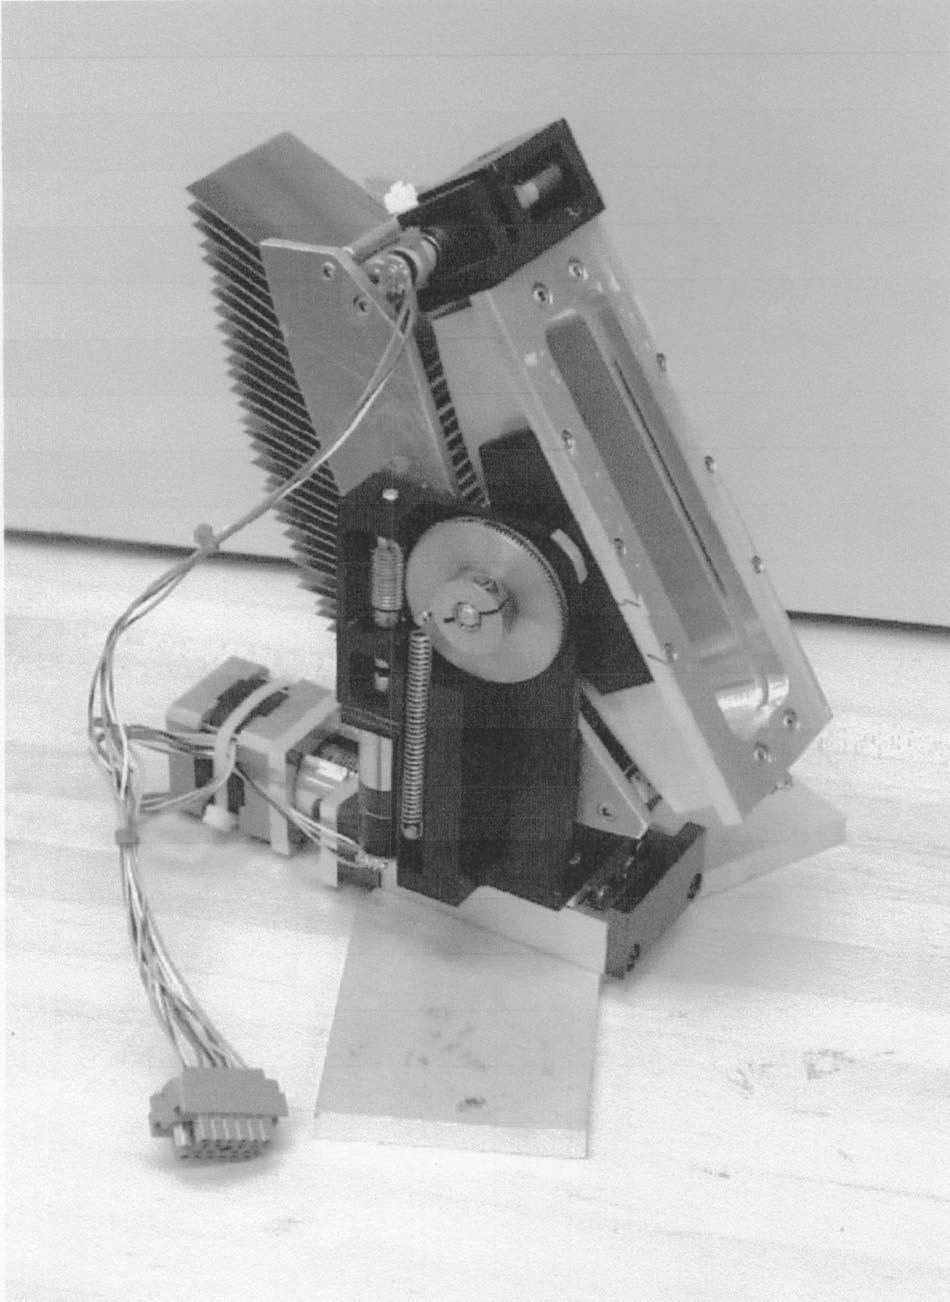
\includegraphics[width=0.9\linewidth]{pses/hires/bla_bw.jpg}
    \end{column}
    \begin{column}{0.35\linewidth}
      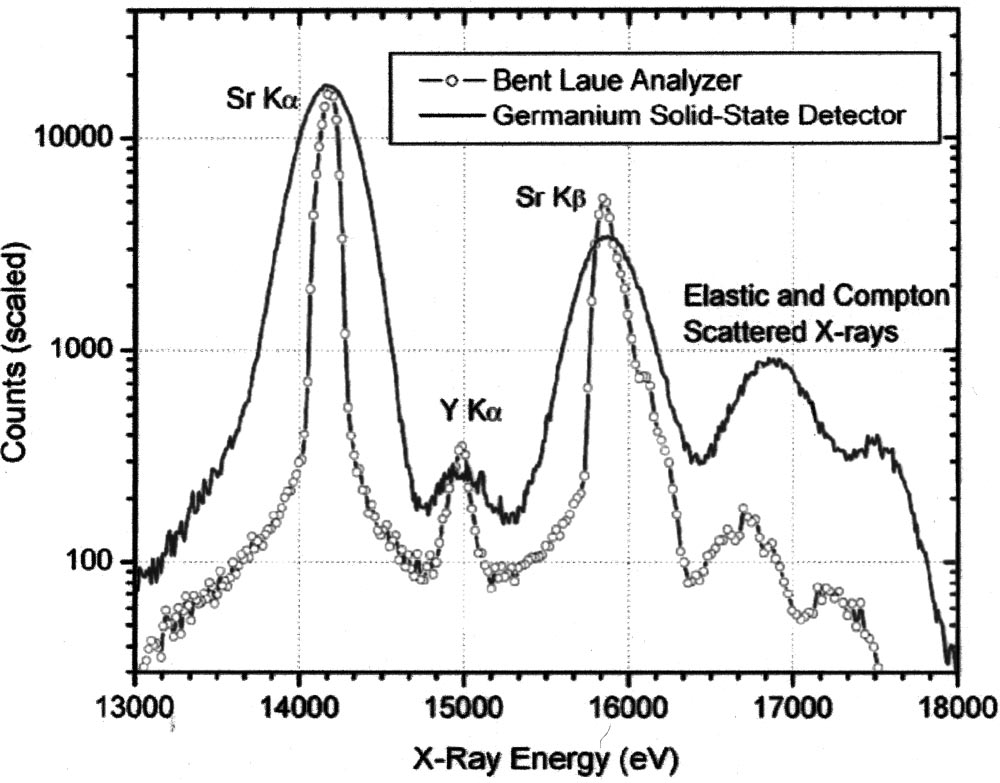
\includegraphics[width=0.9\linewidth]{pses/hires/resolution.png}      
    \end{column}
    \begin{column}{0.35\linewidth}
      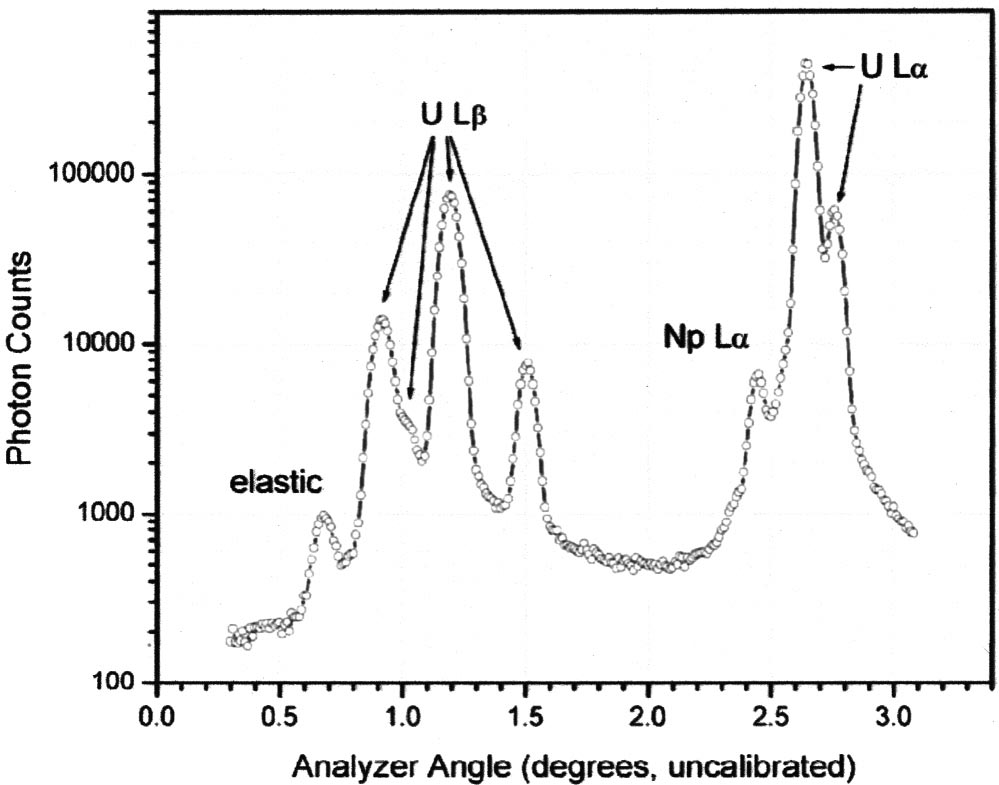
\includegraphics[width=0.9\linewidth]{pses/hires/unp.png}      
    \end{column}
  \end{columns}
  
  \bigskip

  \scriptsize
  ``The signal to background is 3.5:1, even though the Np peak is
  still clearly sitting on the tail of the uranium fluorescence peak
  as in [the figure]. This ratio means that the uranium fluorescence
  has been reduced by about 550 compared to the unfiltered beam. As a
  practical consequence, since reasonably good XAFS spectra can
  generally be obtained in the fluorescence mode for a
  signal-to-background ratio of 1:2, \alert{given enough time}, we could
  theoretically measure XAFS with no change to this configuration for
  a 1:1100 Np to U ratio.''
  \begin{textblock*}{0.6\linewidth}(0pt,19.5\TPVertModule)
    \tiny
    Images and text from A.J.\ Kropf, et al,
    \textit{Rev.\ Sci.\ Instrum.} \textbf{74} (2003) 4696-4702.
  \end{textblock*}
\end{frame}

\begin{frame}
  \frametitle{Scaling up high resolution measurements}
  \begin{columns}
    \begin{column}{0.6\linewidth}
      \begin{center}
        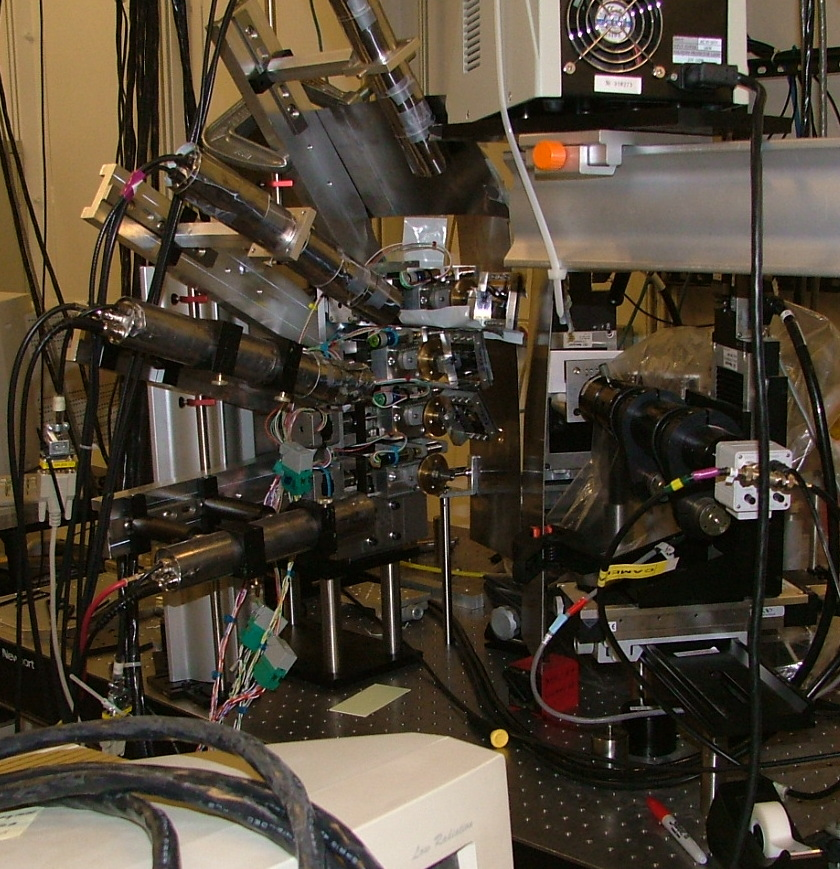
\includegraphics[width=0.8\linewidth]{pses/hires/bla_array.jpg}
      \end{center}
    \end{column}
    \begin{column}{0.4\linewidth}
      \begin{center}
        \scriptsize
        Pt metal: normal and high res.\\
        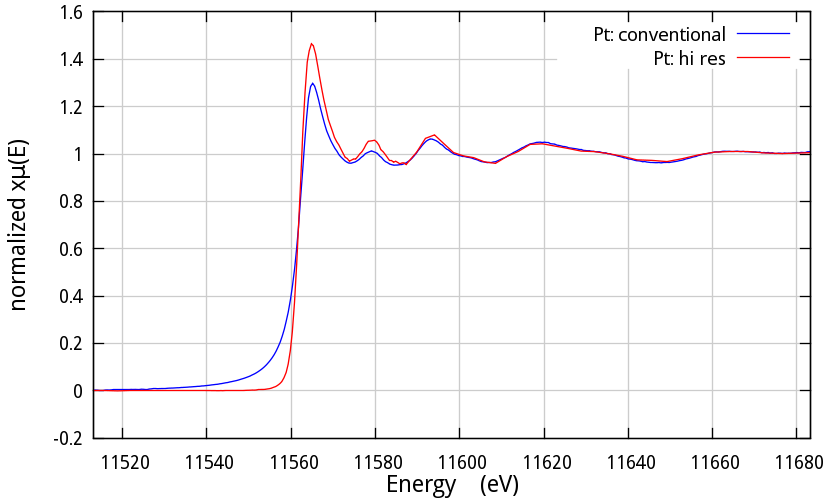
\includegraphics[width=0.95\linewidth]{pses/hires/pt_hi_res.png}\\[3ex]
        U$^{4+}$, U$^{6+}$, and mixed U$^{5+}$/U$^{6+}$
        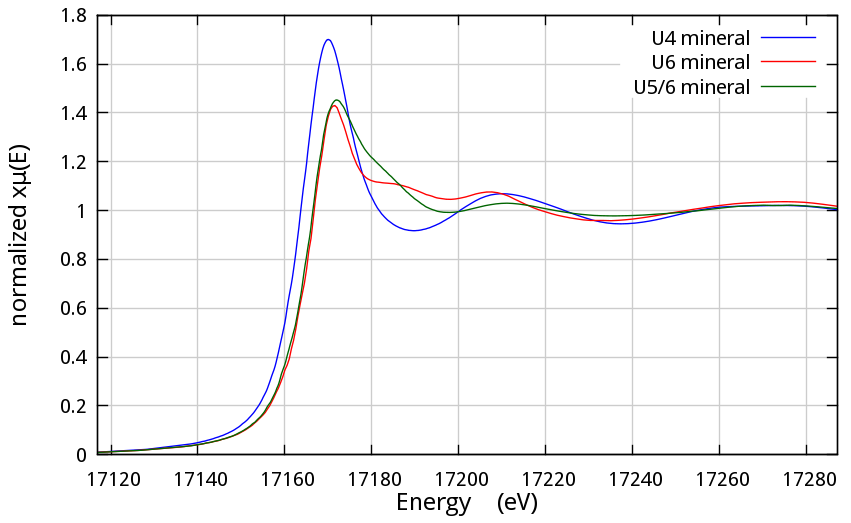
\includegraphics[width=0.95\linewidth]{pses/hires/u456.png}
      \end{center}
    \end{column}
  \end{columns}

  \medskip

  \small
  Many important issues in environmental science require careful
  consideration of valence state.  In the U example, the spectral
  features of the U$^{5+}$ state are difficult to disentangle at
  standard resolution.
  \begin{textblock*}{0.6\linewidth}(0pt,20\TPVertModule) \tiny
    Pt data from A.J.\ Kropf.
  \end{textblock*}
\end{frame}

\subsection[Exotic spectroscopies]{Exotic spectroscopies}

\begin{frame}
  \frametitle{X-ray Emission Spectroscopy}

  Use spherical crystal analyzers to resolve the various fluorescence
  lines.
  
  \begin{center}
    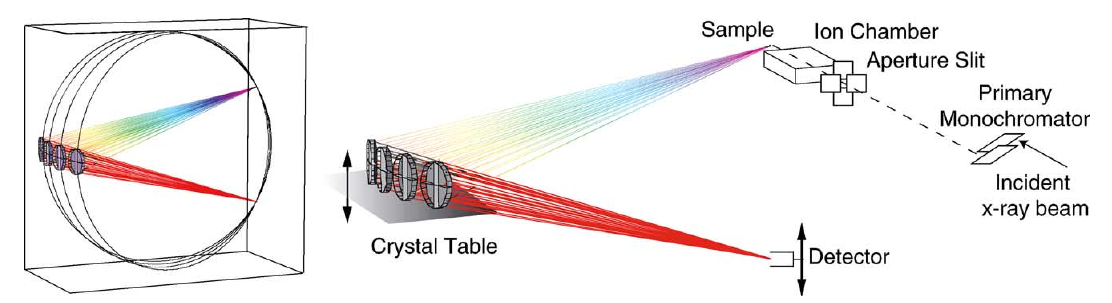
\includegraphics[width=0.9\linewidth]{pses/XES/exp.png}
  \end{center}
  \begin{columns}
    \begin{column}{0.4\linewidth}
      \begin{center}
        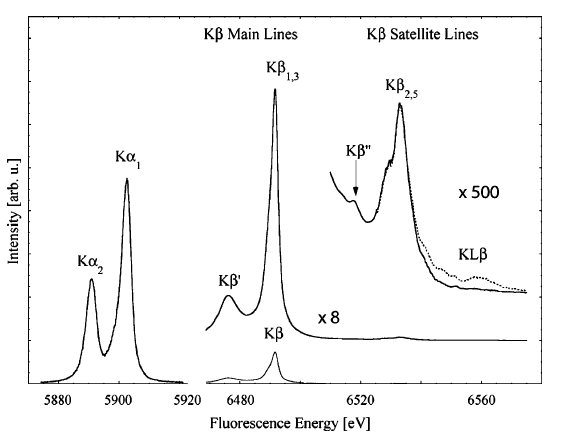
\includegraphics[width=0.9\linewidth]{pses/XES/lines.png}
      \end{center}
    \end{column}
    \begin{column}{0.6\linewidth}
      \begin{center}
        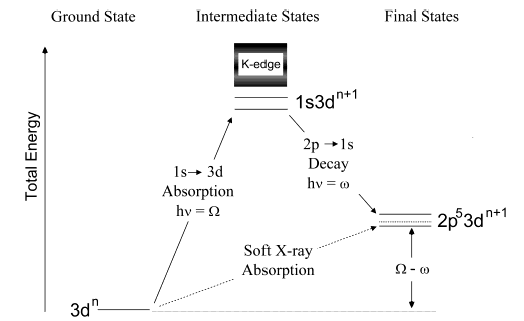
\includegraphics[width=0.8\linewidth]{pses/XES/rixs_schema.png}
      \end{center}
    \end{column}
  \end{columns}
  

  \begin{textblock*}{0.6\linewidth}(0pt,19.5\TPVertModule) \tiny
    P. Glatzel and U. Bergman, \textit{Coordination Chemistry Reviews}
    \textbf{249} (2005) 65–95 and P. Glatzel et al \textit{JACS}
    (2004) \textbf{126}, 9946-9959
  \end{textblock*}
\end{frame}

\begin{frame}
  \frametitle{The RIXS plane}
  \begin{columns}[T]
    \begin{column}{0.3\linewidth}
      \begin{center}
        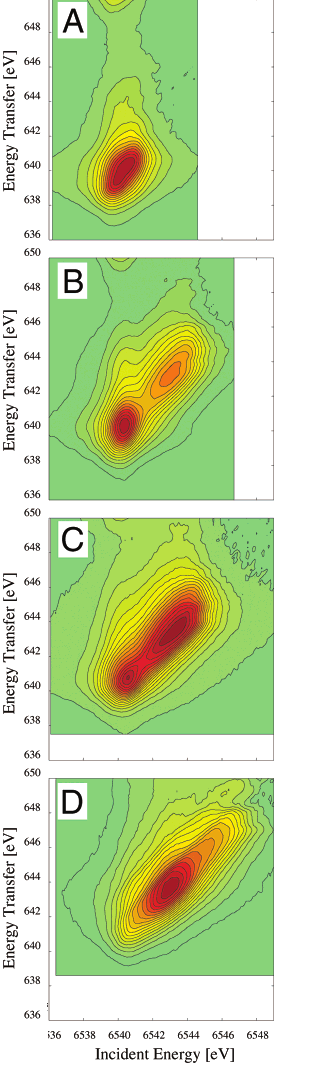
\includegraphics[width=0.7\linewidth]{pses/XES/mn_rixs.png}
      \end{center}
    \end{column}
    \begin{column}{0.7\linewidth}
      1s$^2$p$^{3/2}$ RIXS planes for Mn oxides: (A) MnO, (B)
      Mn$_3$O$_4$, (C) Mn$_2$O$_3$, and (D) MnO$_2$, after subtraction
      of the main edge.

      \begin{center}
        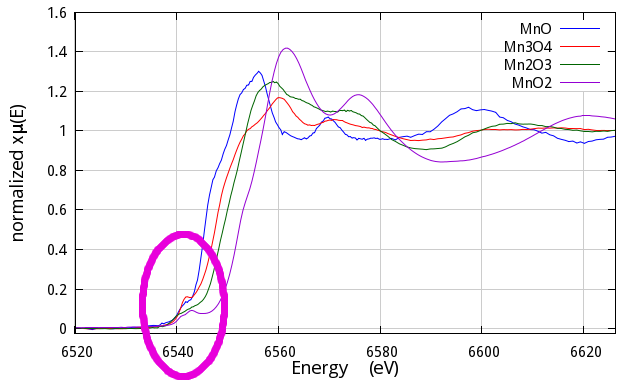
\includegraphics[width=0.7\linewidth]{pses/XES/mn_oxides_xas.png}
      \end{center}

      Substantial differences between the oxides.

      \bigskip

      Note the additional structure in MnO

    \end{column}
  \end{columns}
  \begin{textblock*}{0.6\linewidth}(0pt,19.5\TPVertModule) \tiny
    P. Glatzel and U. Bergman, \textit{Coordination Chemistry Reviews}
    \textbf{249} (2005) 65–95 and P. Glatzel et al \textit{JACS}
    (2004) \textbf{126}, 9946-9959
  \end{textblock*}
\end{frame}

\begin{frame}
  \frametitle{Ligand-selective fluorescence spectroscopy}

  Distinguishing first row scatterers in an XAS measurement is a
  persistent problem in the interpretation of XAS data.

  \begin{columns}
    \begin{column}{0.5\linewidth}
      \begin{center}
        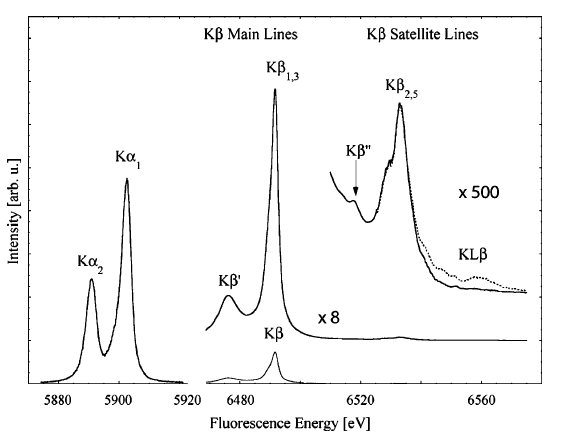
\includegraphics[width=0.9\linewidth]{pses/XES/lines.png}
      \end{center}
    \end{column}
    \begin{column}{0.5\linewidth}
      \begin{center}
        K$\beta''$ and K$\beta_{2,5}$ lines of Mn\\
        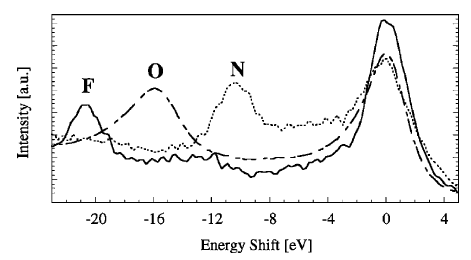
\includegraphics[width=\linewidth]{pses/XES/ligand.png}
      \end{center}
    \end{column}
  \end{columns}
  \begin{exampleblock}{Ligand sensitive signal!}
    The K$\beta''$ line is ligand-sensitive, but it is also down from
    the K$\alpha$ signal by 3 orders of magnitude.  One needs lots of
    photons!
  \end{exampleblock}

  \begin{textblock*}{0.6\linewidth}(0pt,19.5\TPVertModule)
    \tiny
    P. Glatzel and U. Bergman, \textit{Coordination Chemistry Reviews}
    \textbf{249} (2005) 65–95 and P. Glatzel et al \textit{JACS}
    (2004) \textbf{126}, 9946-9959
  \end{textblock*}
\end{frame}

\begin{frame}
  \frametitle{LERIX: Lower Energy Resonant Inelastic Scattering}

  Probe the sample with hard x-rays and use the crystal analyzers to
  resolve the energy loss in the nearly-elastically scattered
  radiation due to absorption by low-energy edges.

  \medskip

  \begin{columns}
    \begin{column}{0.5\linewidth}
      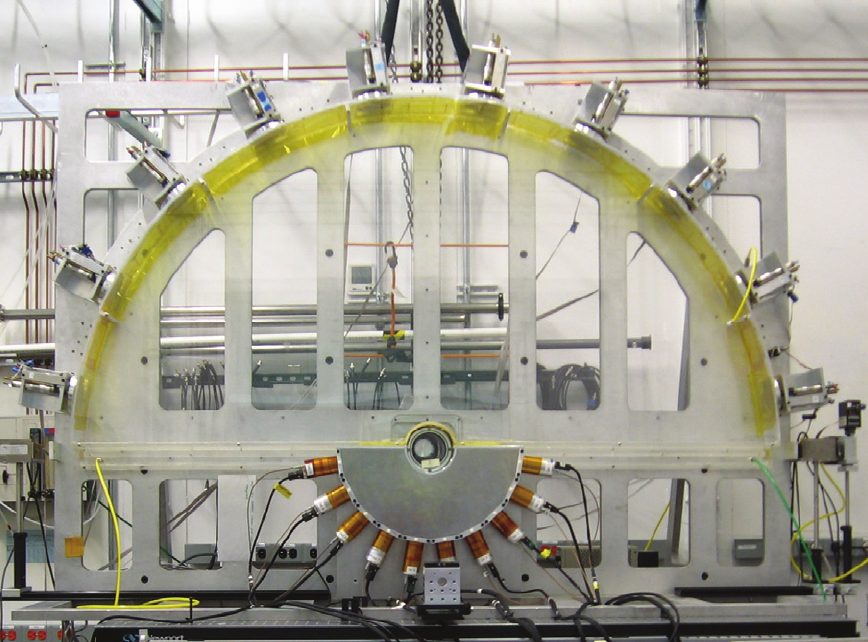
\includegraphics[width=0.9\linewidth]{pses/lerix/instrument.png}
    \end{column}
    \begin{column}{0.5\linewidth}
      \qquad C K-edge of Diamond\\
      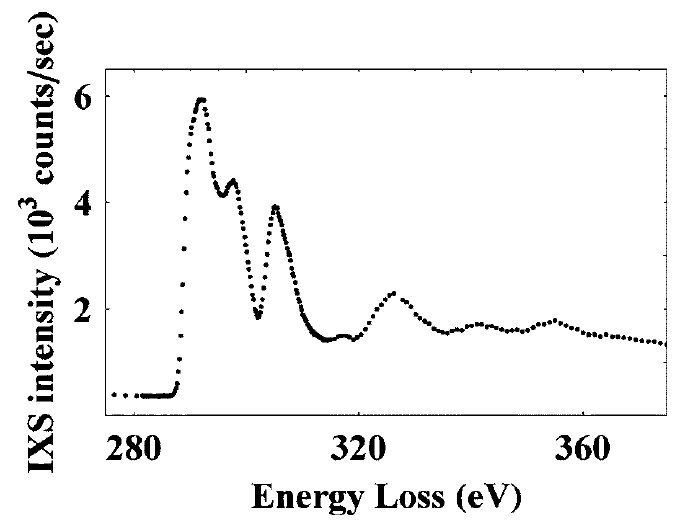
\includegraphics[width=0.9\linewidth]{pses/lerix/diamond.png}      
    \end{column}
  \end{columns}

  \smallskip

  \begin{exampleblock}{Soft x-ray edges measured with hard x-rays!}
    Imagine measuring, for instance, the C k-edge of a wet sample.
  \end{exampleblock}

  \begin{textblock*}{0.6\linewidth}(0pt,19.5\TPVertModule) \tiny
    \tiny
    T.T.\ Fister et al, \textit{Rev.\ Sci.\ Instrum.}
    \textbf{77}, 063901 2006 and G.T.\ Seidler, et al, in X-ray
    Absorption Fine Structure: XAFS13 (AIP Conf.\ Proc.\ 882,
    Eds.\ B.\ Hedman, P.\ Pianetta), p. 911 (2006).
  \end{textblock*}
\end{frame}

\section[Conclusion]{Conclusion}
\begin{frame}
  \frametitle{Conclusion}

  Third generation synchrotron sources along with new developments in
  optics and detectors enable new opportunities for the environmental
  sciences.

  \bigskip

  \begin{itemize}
  \item Many of the things I have discussed are already available at
    synchrotrons in North America and elsewhere in the world.
  \item NSLS-II will bring these exciting new capabilities to those of
    us in the Northeast.
  \end{itemize}

  \bigskip

  \begin{exampleblock}{Your job?}
    Imagine exciting new experiments to make use of these novel capabilities.
  \end{exampleblock}
\end{frame}


\end{document}

%%% Local Variables:
%%% TeX-parse-self: t
%%% TeX-auto-save: t
%%% TeX-auto-untabify: t
%%% TeX-PDF-mode: t
%%% End:
